% Gemini theme
% https://github.com/anishathalye/gemini

\documentclass[final]{beamer}

\usepackage[T1]{fontenc}
\usepackage{lmodern}
\usepackage[size=custom,width=120,height=72,scale=1.0]{beamerposter}
\usetheme{gemini}
\usepackage[numbers, sort&compress]{natbib}
\usecolortheme{cwru}
\usepackage{graphicx}
\usepackage[caption=false]{subfig}
\usepackage{capt-of}
\usepackage{booktabs}
\usepackage{amsmath, amssymb}
\usepackage{tikz}
\usetikzlibrary{bayesnet, plotmarks, matrix}
\usepackage{pgfplotstable}
\usepackage{pgfplots}
\usepgfplotslibrary{groupplots, statistics}
\pgfplotsset{compat=1.15}
% Box plots
\pgfplotsset{
	only if/.style args={entry of #1 is #2}{
		/pgfplots/boxplot/data filter/.code={
			\edef\tempa{\thisrow{#1}}
			\edef\tempb{#2}
			\ifx\tempa\tempb
			\else
			\def\pgfmathresult{}
			\fi
		}
	}
}

% If you have N columns, choose \sepwidth and \colwidth such that
% (N+1)*\sepwidth + N*\colwidth = \paperwidth
\newlength{\sepwidth}
\newlength{\colwidth}
\setlength{\sepwidth}{0.025\paperwidth}
\setlength{\colwidth}{0.3\paperwidth}

\newcommand{\separatorcolumn}{\begin{column}{\sepwidth}\end{column}}

\newcommand{\sval}{r}
\newcommand{\reach}{m_{\theta}}
\newcommand{\estreach}{\hat{m}_{\theta}}

\title{ShareTrace: Contact Tracing with Asynchronous, Parallel Message Passing on a Temporal Graph}

\author{Ryan Tatton \and Erman Ayday \and Youngjin Yoo \and Anisa Halimi}

\institute[shortinst]{Case Western Restern Reserve University}

\footercontent{
  \href{https://github.com/share-trace}{https://github.com/share-trace} \hfill
  Conference on Health, Inference, and Learning (CHIL) 2022 \hfill
  \href{mailto:ryan.tatton.edu}{ryan.tatton@case.edu}}

\begin{document}
\begin{frame}[t]
\begin{columns}[t]
\separatorcolumn
\begin{column}{\colwidth}
	\begin{block}{1. Motivation}
		\begin{itemize}
			\item Proximity-based contact tracing relies on user device interaction to estimate infection spread.
			\item ShareTrace is a privacy-preserving, proximity-based contact-tracing solution that estimates a person's marginal posterior probability of infection (\emph{exposure score}) via iterative message passing on a factor graph based on their prior probability of infection (\emph{symptom score}) and (in)direct contact with others.
			\item The scalability and efficiency of the original ShareTrace algorithm (\emph{risk propagation}) \cite{Ayday2021} can be improved with asynchronous, non-iterative message passing on a temporal graph.
		\end{itemize}
	\end{block}
	\begin{block}{2. Proposed Scheme}
		\begin{itemize}
			\item Reformulate the factor graph as a temporal contact graph of user nodes (Figure \ref{fig:temporal-graph}).
			\item Partition the temporal graph, where each subgraph is an \emph{actor} \cite{Agha1986} that can pass messages.
			\item Actors compute and non-iteratively pass messages (\emph{risk scores}) until a stopping condition is met.
			\item Only propagate messages if they are likely to affect other users' exposure scores in the graph.
			\item \emph{Send tolerance} $\gamma$ parametrizes the trade-off between completeness and efficiency of asynchronous, non-iterative message passing. A user node $u$ only propagates a risk score if it is sufficiently high (by a factor of $\gamma$) and sufficiently old (relative to the initial message sent by $u$).
		\end{itemize}
		\begin{figure}
			\centering
			\resizebox{0.75\columnwidth}{!}{%
				\begin{tikzpicture}[baseline={(0,0)}, ampersand replacement=\&]
					\matrix[row sep=1em, column sep=-0.5em] at  (-4, 0)
					{%
						\& \factor[minimum size=0.5em] {f12} {above:$f(v_1, v_2)$} {} {}; \&\&
						\factor[minimum size=0.5em] {f23} {above:$f(v_2, v_3)$} {} {}; \& \\
						\node[latent, label=below:$v_1$, minimum size=1em] (v1) {}; \&\&
						\node[latent, label=below:$v_2$, minimum size=1em] (v2) {}; \&\&
						\node[latent, label=below:$v_3$, minimum size=1em] (v3) {}; \\
					};
					\edge[-] {v1} {f12};
					\edge[-] {v2} {f12};
					\edge[-] {v2} {f23};
					\edge[-] {v3} {f23};
					$\implies$
					\matrix[row sep=4em, column sep=2em] at (6, 0)
					{%
						\node[latent, label=below:$v_1$, minimum size=1em] (v1) {}; \& 
						\& \node[latent, label=below:$v_3$, minimum size=1em] (v3) {}; \\
						\& \node[latent, label=below:$v_2$, minimum size=1em] (v2) {}; \& \\
					};
					\factor[minimum size=0.5em, above= of v1] {f121} {above:$f(v_1, v_2)$} {} {};
					\factor[minimum size=0.5em, above= of v2, xshift=-1.5em] {f122} {above:$f(v_1, v_2)$} {} {};
					\factor[minimum size=0.5em, above= of v2, xshift=1.5em] {f232} {above:$f(v_2, v_3)$} {} {};
					\factor[minimum size=0.5em, above= of v3] {f233} {above:$f(v_2, v_3)$} {} {};
					
					\plate{p1} {(v1)(f121)(f121-caption)} {$u_1$};
					\plate{p2} {(v2)(f122)(f232)(f122-caption)(f232-caption)} {$u_2$};
					\plate{p3} {(v3)(f233)(f233-caption)} {$u_3$};
					
					\edge[-] {v1} {f121};
					\edge[-] {v2} {f122};
					\edge[-] {v2} {f232};
					\edge[-] {v3} {f233};
					\edge[-] {p1} {p2};
					\edge[-] {p2} {p3};
				\end{tikzpicture}
			}%
			\caption{A factor graph of 3 variables and 2 factors (left) as a temporal contact graph of 3 users (right).}
			\label{fig:temporal-graph}
		\end{figure}
	\end{block}
	\begin{block}{3. Message Reachability (MR)}
		\begin{itemize}
			\item The \emph{estimated MR} $\estreach$ is a measure to characterize the propagation of risk as a dynamic process on a temporal graph \cite{Barrat2013}, i.e. the number of users a user can impact with their risk.
			\item Parametrized by $\theta$, which includes the transmission rate $\alpha$, the send tolerance $\gamma$, the initial risk score $r_u$ of user $u$, and the initial risk score $r_v$ of some reachable user $v$ from $u$:
				\begin{equation} \label{eq:msg-reach}
					 \alpha^{\estreach(u)} \sval_u \leq \gamma \alpha \sval_v \implies \estreach(u)
					 	\leq 1 + \log_{\alpha}\left(\frac{\gamma \sval_v}{\sval_u}\right)
				\end{equation}
			\item The \emph{actual MR} $\reach$ can be found by applying an augmented shorted-path algorithm with message passing, which accounts for the temporality of contacts.
			\item A user $v$ is \emph{message-reachable} from user $u$ if there exists a path from $u$ to $v$ such that all users along the path satisfy \eqref{eq:msg-reach} and the risk score of $u$ is within $B$ days of each contact.
		\end{itemize}
	\end{block}
\end{column}
\separatorcolumn
\begin{column}{\colwidth}
	\begin{block}{4. Experimental Design}
		\begin{itemize}
			\item Synthetic graphs included random geometric graphs (RGG) \cite{Dall2002}, benchmark graphs (LFRG) \cite{Lancichinetti2008}, and clustered scale-free graphs (CSFG) \cite{Holme2002}. See Figure \ref{fig:sociopatterns} regarding real-world graphs.
			\item METIS was used to partition the graphs with a load imbalance factor of 0.2 and set to attempt contiguous partitions and minimize the connectivity between partitions \cite{Karypis1998}.
			\item Users were assigned ``high'' risk (scores above 0.5) with probability 0.2, and ``low'' risk otherwise.
			\item Default parameter values: transmission rate $\alpha = 0.8$; send tolerance $\gamma = 0.6$.
			\item We ran 10 trials for each synthetic (real-world) graph for MR (resp. scalability) experiments.
		\end{itemize}
	    \begin{figure}
	    	\centering
	    	\subfloat[High school (Thiers13): 180 / 2,220]
	    		{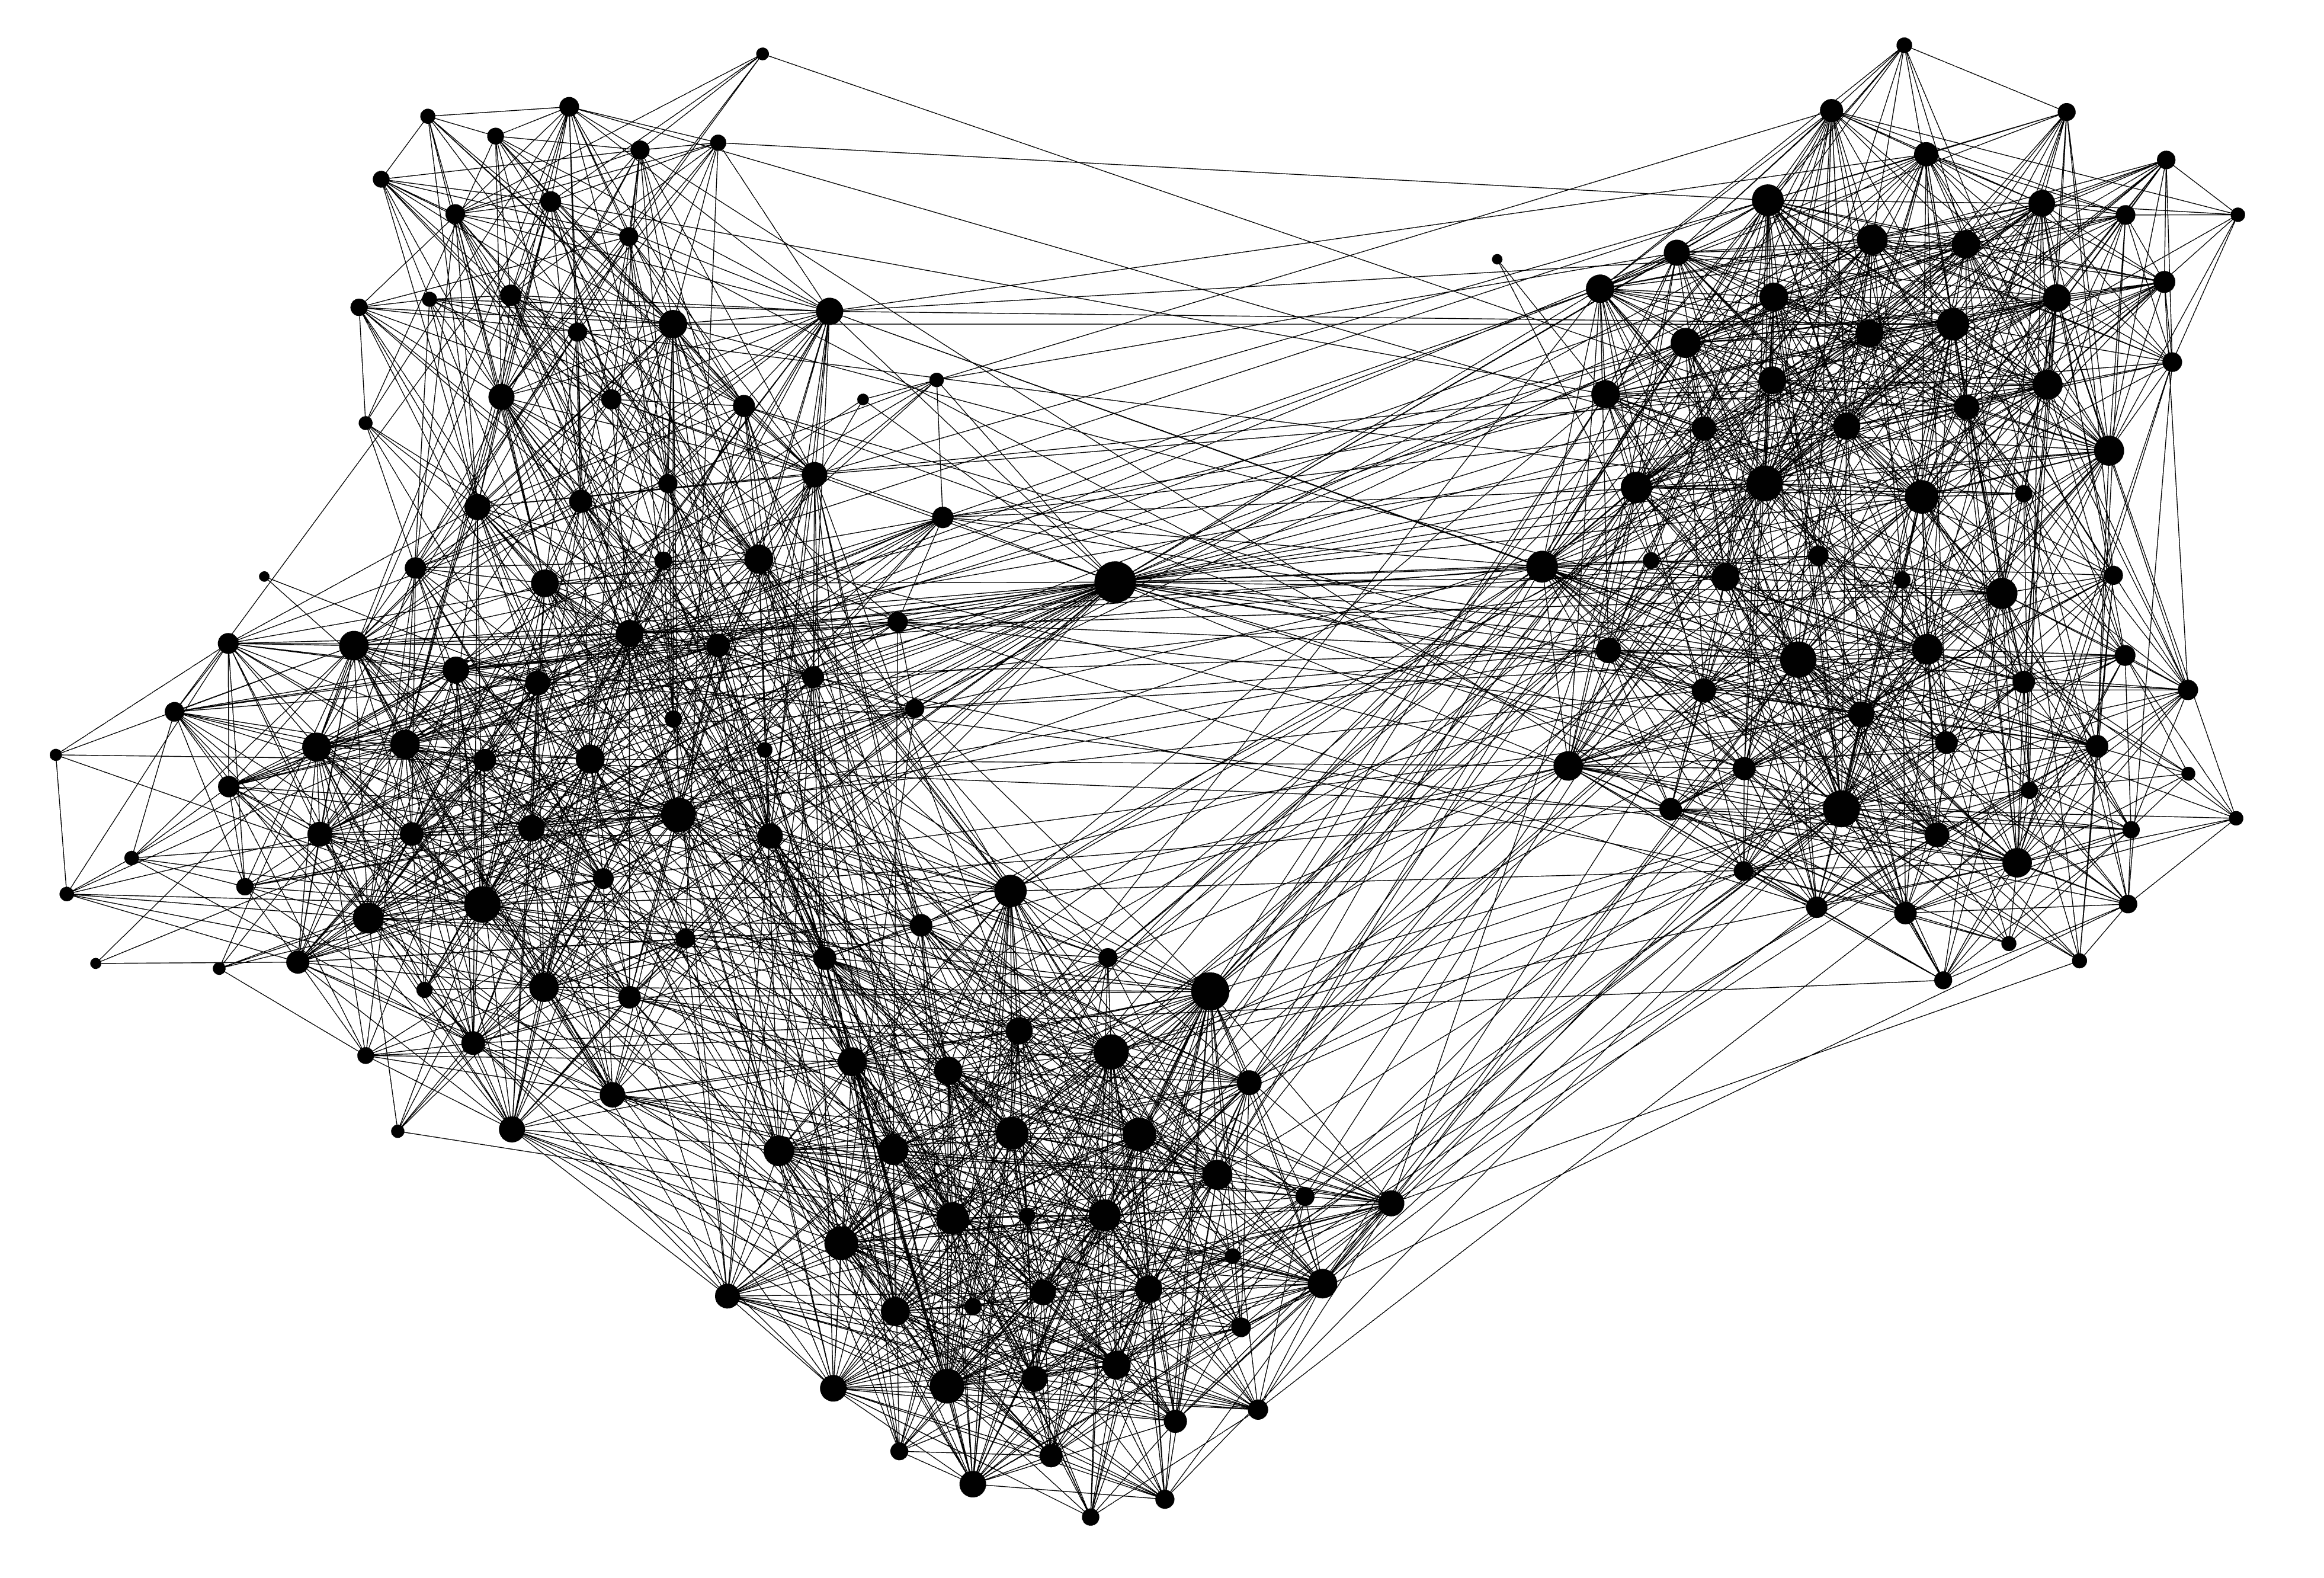
\includegraphics[width=0.3\columnwidth]{contact-tracing/evaluation/figures/highschool12}} \qquad
			\subfloat[Workplace (InVS15): 217 / 4,274]
				{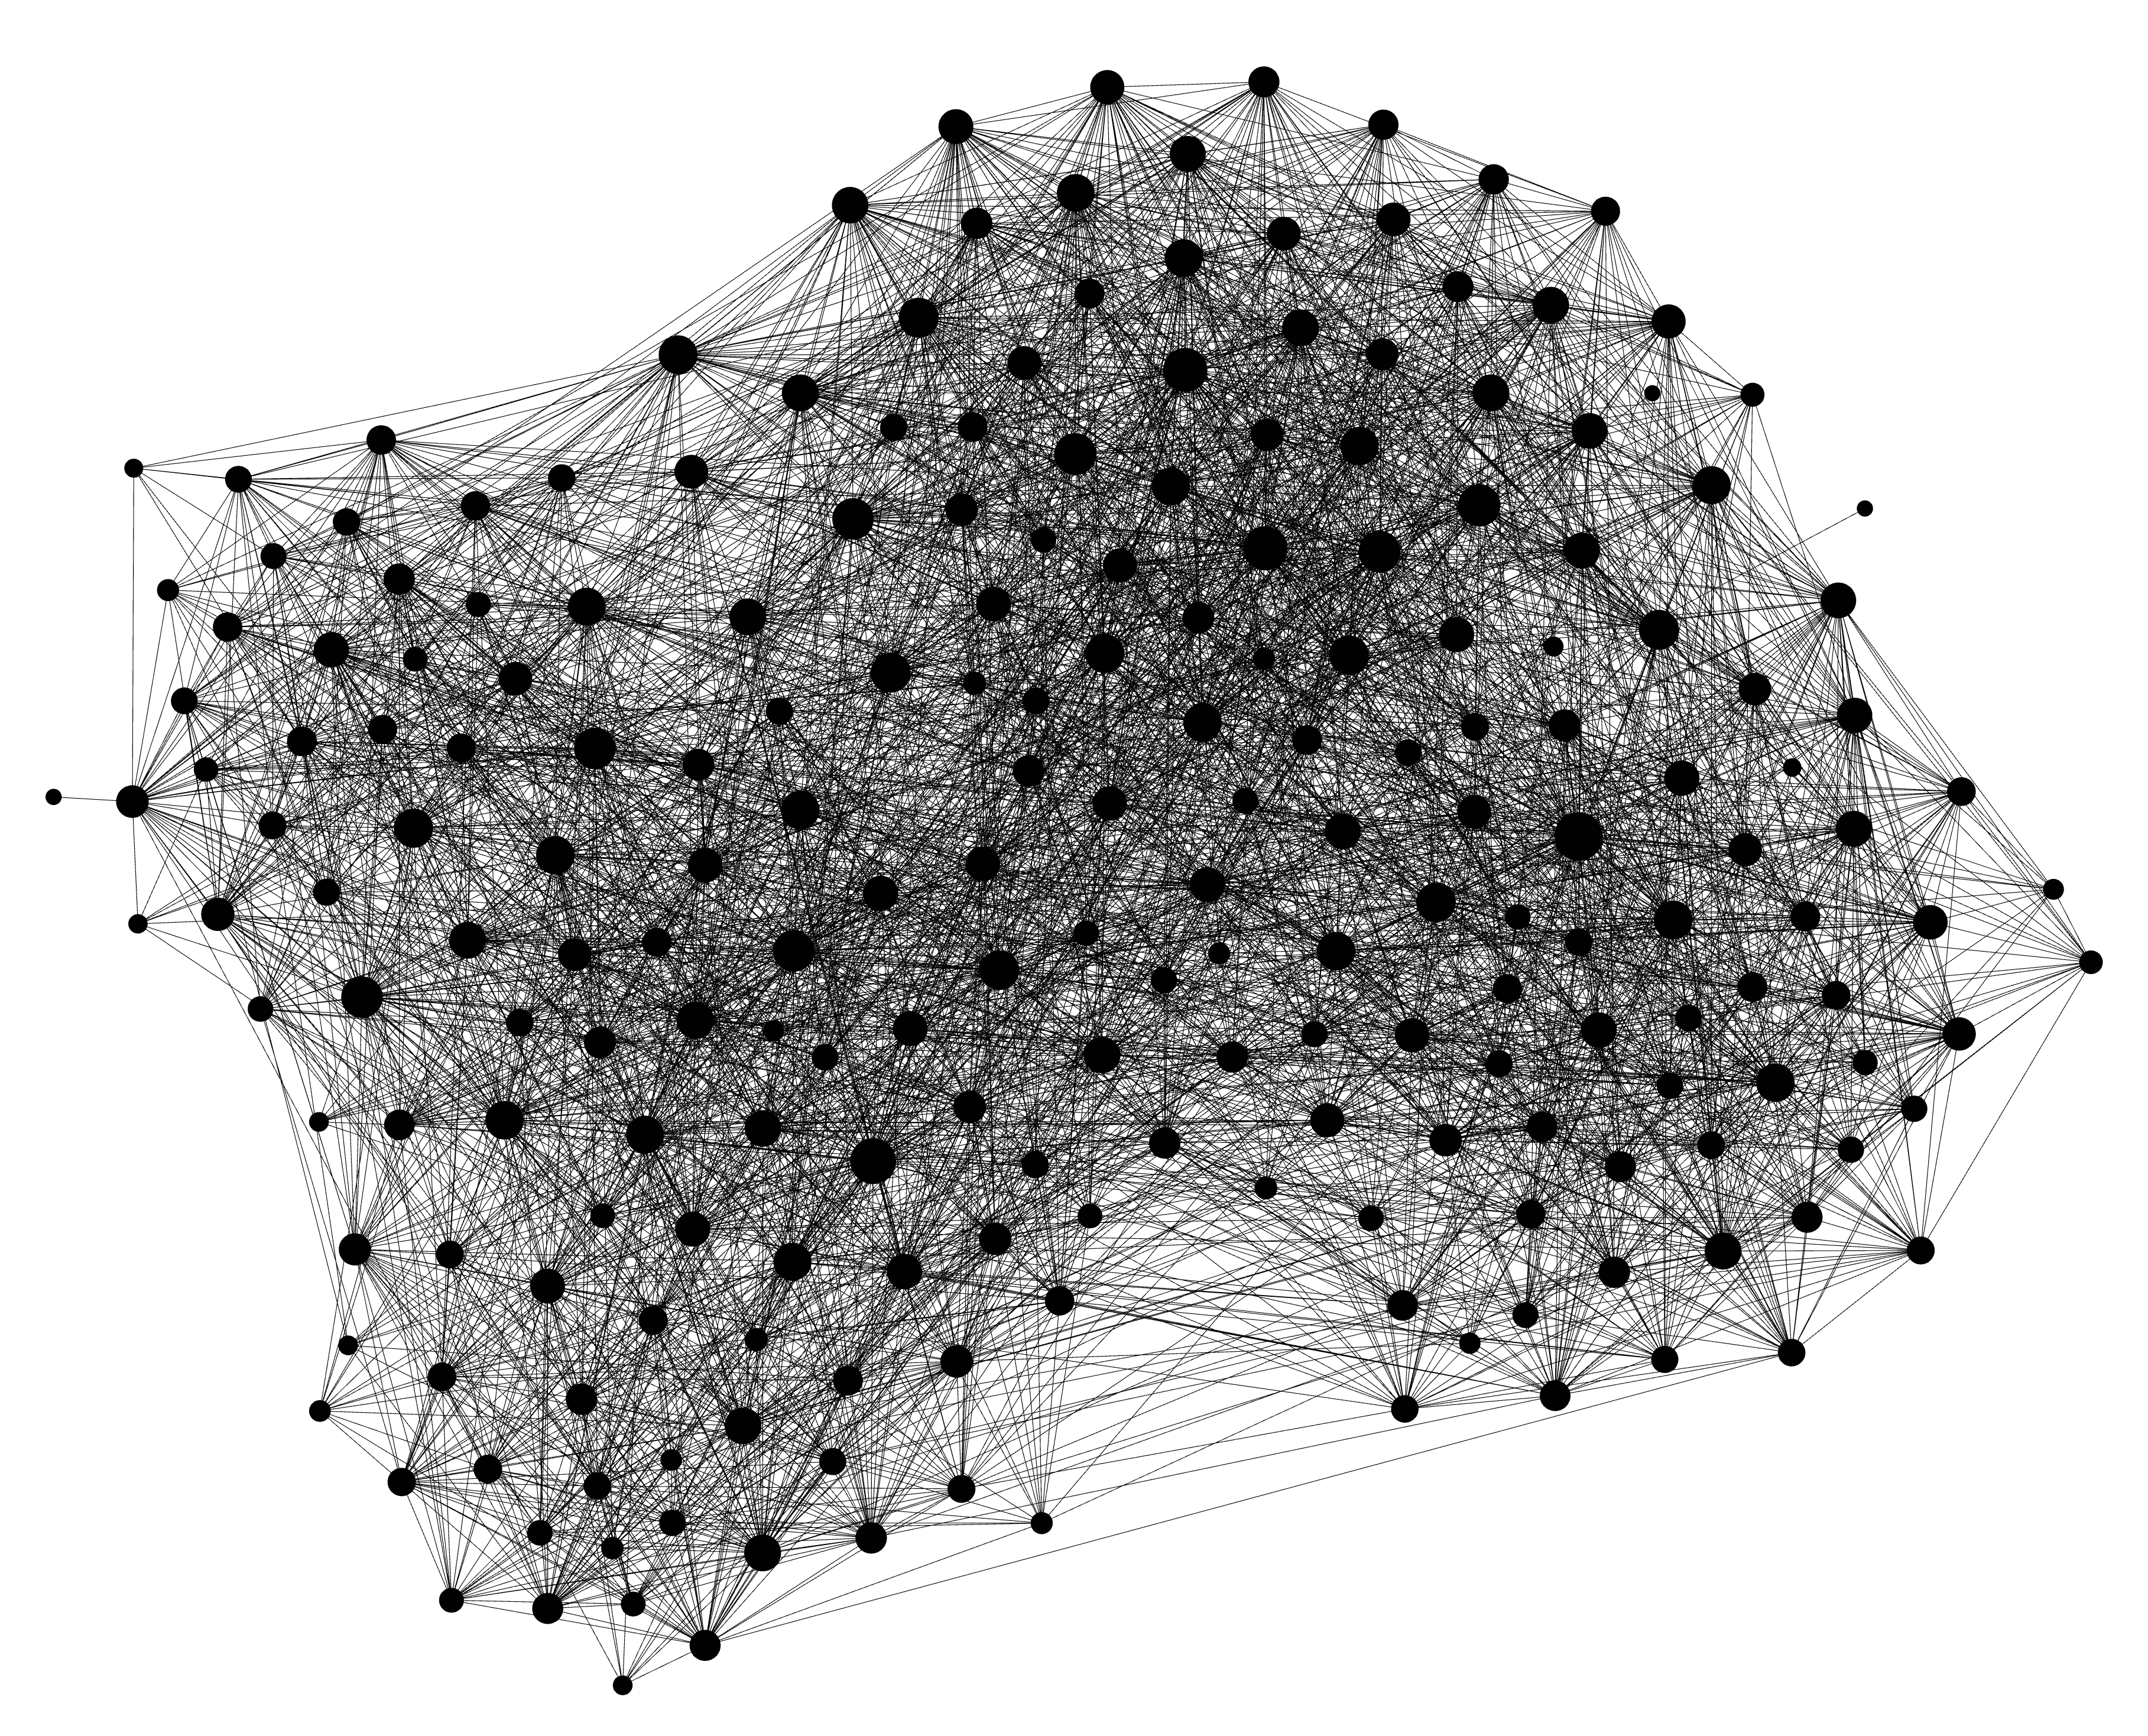
\includegraphics[width=0.3\columnwidth]{contact-tracing/evaluation/figures/workplace}} \qquad
			\subfloat[Scientific conf. (SFHH): 403 / 9,565]
				{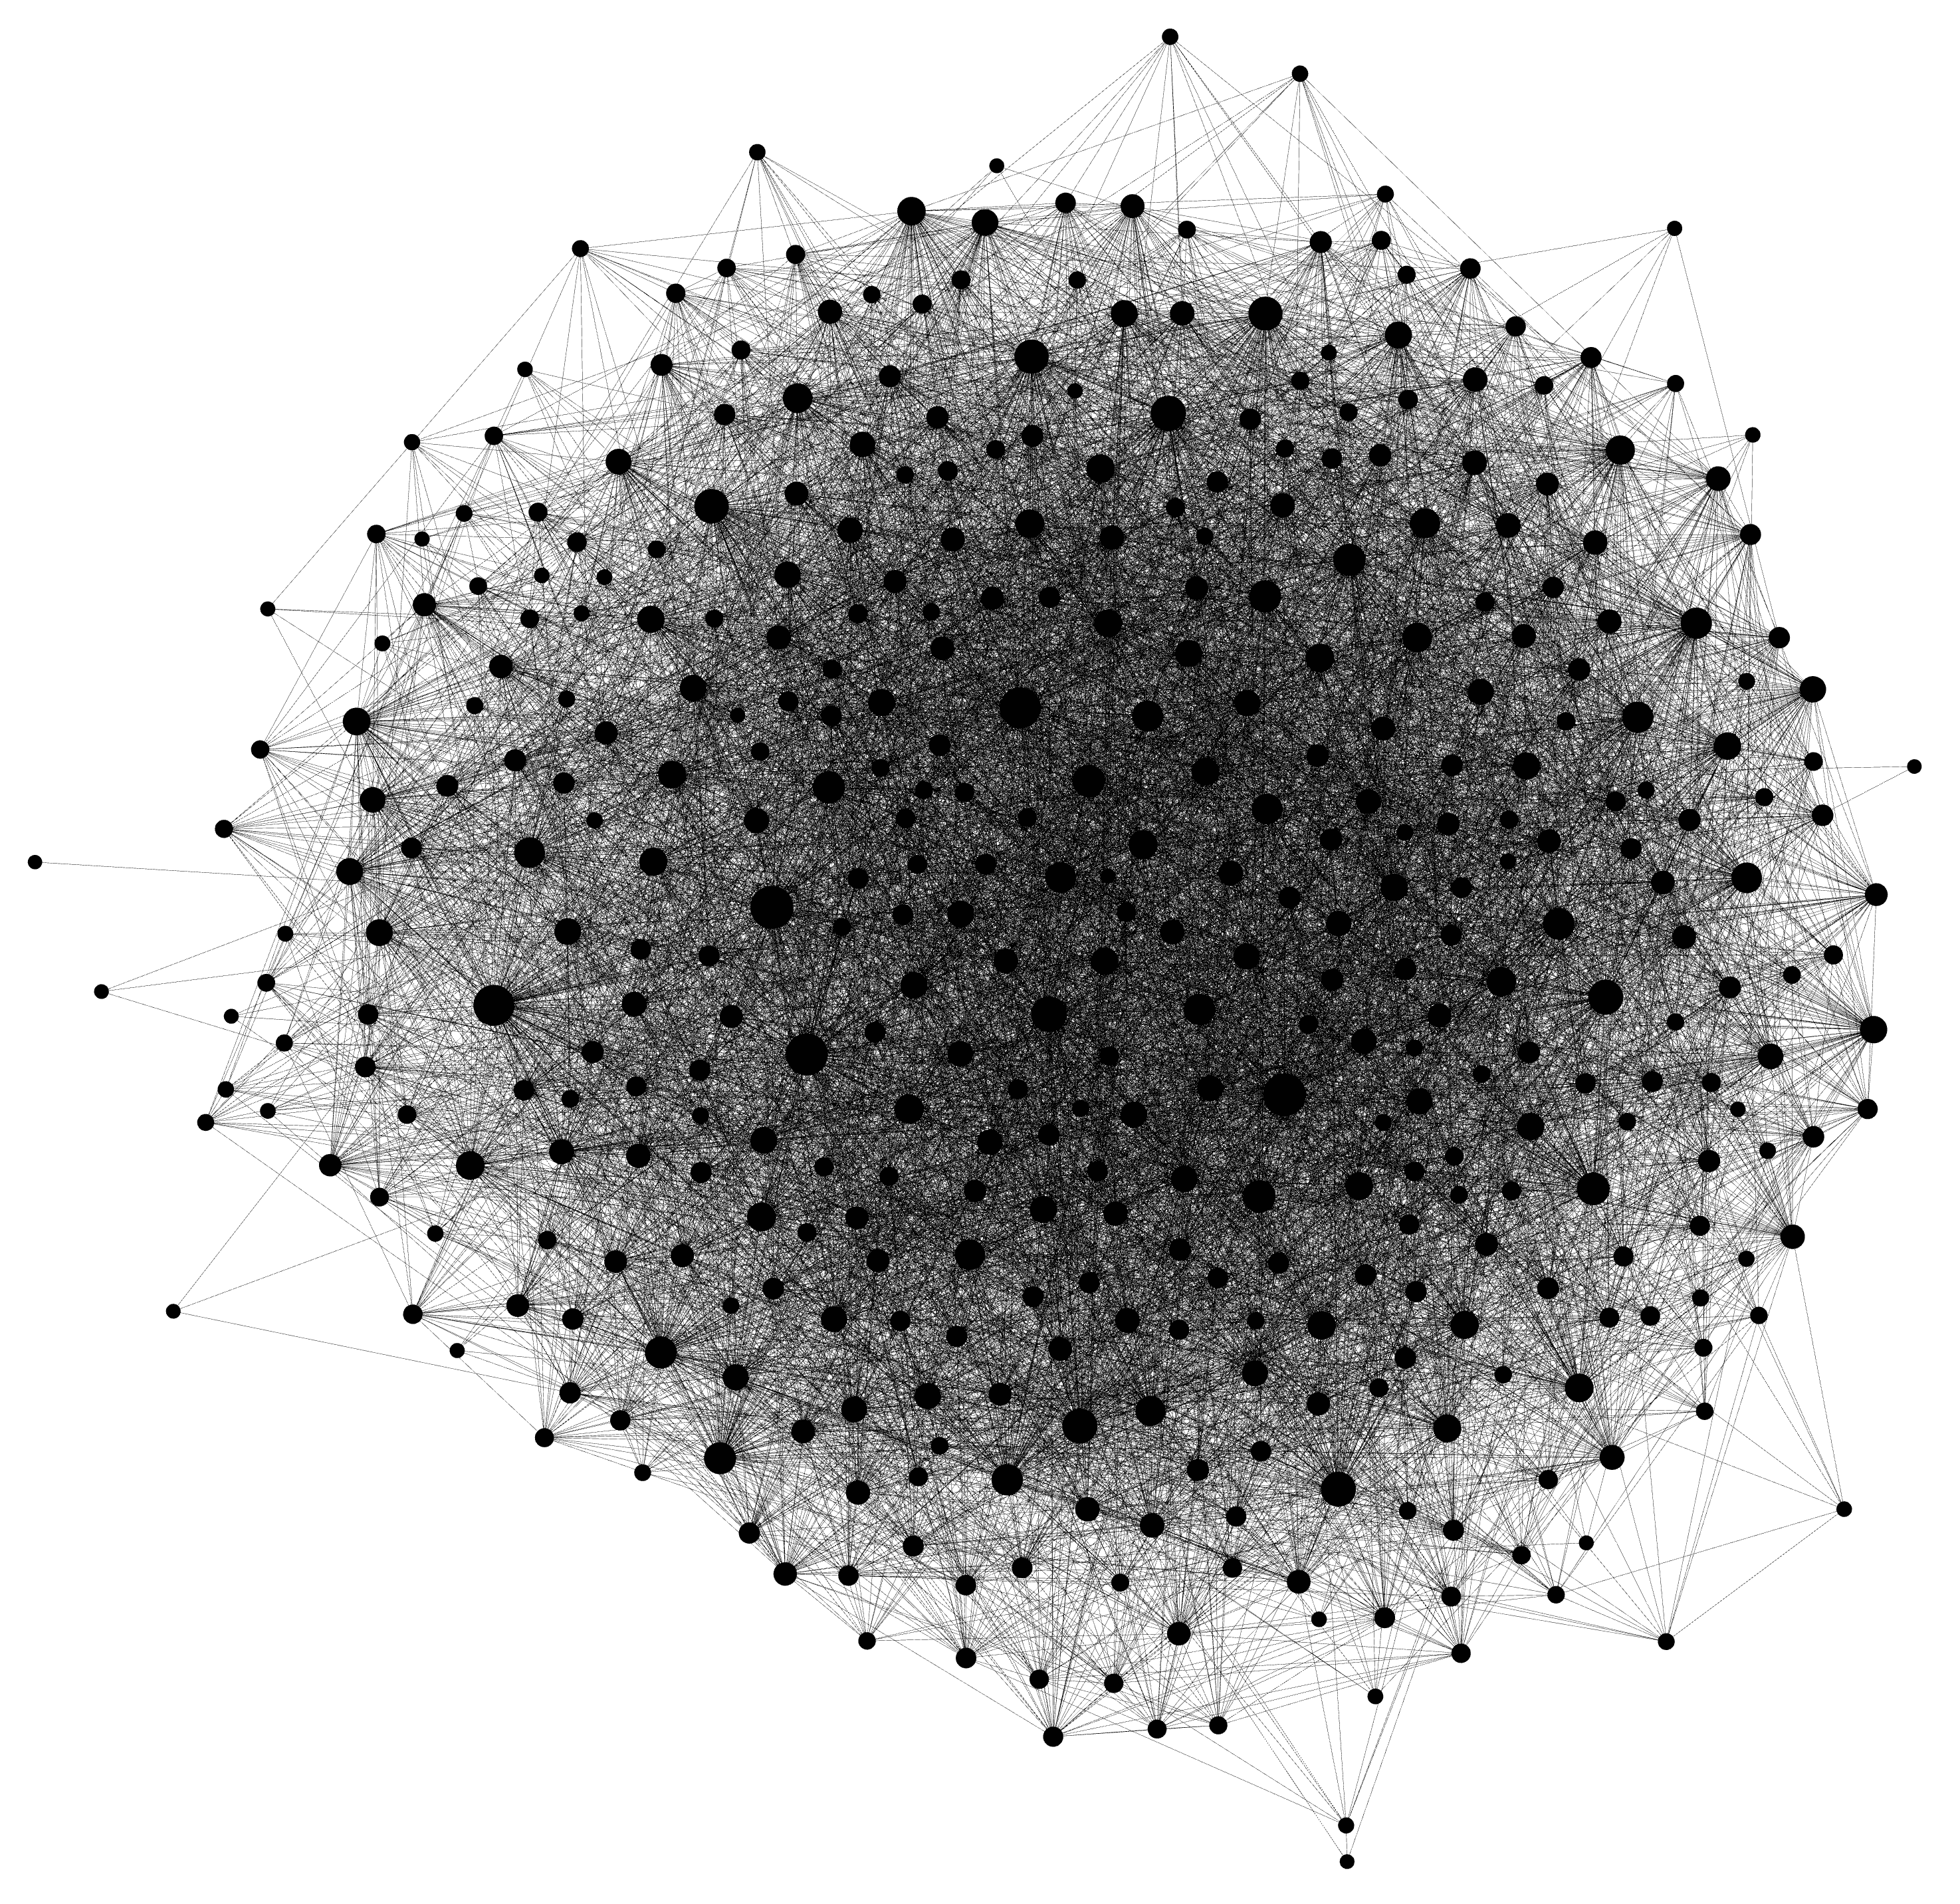
\includegraphics[width=0.3\columnwidth]{contact-tracing/evaluation/figures/conference}}
			\caption{SocioPatterns contact graphs (number of users / number of contacts) \cite{Genois2018}. Each edge represents the most recent time of contact (duration of at least 20 seconds) between two users.}
			\label{fig:sociopatterns}
		\end{figure}
	\end{block}
	\begin{block}{5. Efficiency Results}
		\begin{itemize}
			\item We evaluated the effects of transmission rate and send tolerance on risk propagation efficiency using synthetic graphs with 5,000 users and 2 actors.
			\item A send tolerance of $\gamma = 0.6$ optimizes for completeness and efficiency by permitting 99\% of the possible user updates, while resulting in faster runtimes, $(Q_1, Q_2, Q_3) = (0.13, 0.13, 0.46)$, and fewer messages, $(Q_1, Q_2, Q_3) = (0.13, 0.15, 0.44)$, for a transmission rate of $\alpha = 0.8$.
		\end{itemize}
		\begin{figure}
			\centering
			\resizebox{\columnwidth}{!}{%
				\begin{tikzpicture}
					\begin{groupplot}[
						group style={
						group size=3 by 1,
						xlabels at=edge bottom,
						y descriptions at=edge left
					},
					boxplot,
					table/col sep=comma,
					boxplot/draw direction=y, 
					scaled x ticks={base 10:-1},
					width=0.3\columnwidth,
					height=0.3\columnwidth,
					ytick distance=0.2,
					xtick scale label code/.code={},
					xlabel={Send tolerance, $\gamma$}
				]
					\nextgroupplot[table/y=NormalizedUpdates, title={Normalized updates}]
						\foreach \t in {1,...,10} {%
							\addplot[color=black] table[only if={entry of SendTolerance is \t}]
							{contact-tracing/evaluation/figures/tolerance-updates.csv};
						}%
					\nextgroupplot[table/y=NormalizedRuntimeInSeconds, title={Normalized runtime}]
						\foreach \t in {1,...,10} {%
							\addplot[color=black] table[only if={entry of SendTolerance is \t}]
							{contact-tracing/evaluation/figures/tolerance-runtime.csv};
						}%
						\nextgroupplot[table/y=NormalizedMessages, title={Normalized messages}]
						\foreach \t in {1,...,10} {%
							\addplot[color=black] table[only if={entry of SendTolerance is \t}]
							{contact-tracing/evaluation/figures/tolerance-messages.csv};
						}%
					\end{groupplot}
				\end{tikzpicture}
			}%
			\caption{Effects of send tolerance and transmission rate on efficiency. All dependent variables are normalized across graphs and transmission rates. Efficiency on LFRGs were less sensitive to changes in transmission rate and send tolerance than RGGs and CSFGs, which is the cause for the large interquartile ranges.}
		\end{figure}
	\end{block}
\end{column}
\separatorcolumn
\begin{column}{\colwidth}
	\begin{block}{6. Message Reachability Results}
		\begin{itemize}
			\item Equation \eqref{eq:msg-reach} was a better estimator on synthetic graphs, compared to real-world graphs (Table \ref{table:reach}).
			\item With lower (higher) send tolerances (resp. transmission rates), \eqref{eq:msg-reach} suggests higher MR; however, a message is only passed under certain conditions, so \eqref{eq:msg-reach} tends to overestimate $\reach$.
		\end{itemize}
		\begin{table}
			\begin{minipage}[b]{0.66\columnwidth}
				\centering
					\begin{tikzpicture}
						\begin{groupplot}[
							group style={
								group size=2 by 1,
								xlabels at=edge bottom,
								y descriptions at=edge left
							},
							boxplot,
							title={A/E MRR, $\reach / \estreach$},
							table/col sep=comma,
							boxplot/draw direction=y,    
							xtick distance=2,
							scaled x ticks={base 10:-1},
							xtick scale label code/.code={},
							ytick distance=0.5,
							width=0.5\columnwidth,
							height=0.5\columnwidth
							]
							\nextgroupplot[table/y=RatioValue, xlabel={Send tolerance, $\gamma$}]
							\foreach \t in {1,...,10} {%
								\addplot[color=black] table[only if={entry of SendTolerance is \t}]
								{contact-tracing/evaluation/figures/ratio-tolerance.csv};
							}%
							\nextgroupplot[table/y=RatioValue, xlabel={Transmission rate, $\alpha$},]
							\foreach \t in {1,...,9} {%
								\addplot[color=black] table[only if={entry of Transmission is \t}]
								{contact-tracing/evaluation/figures/ratio-transmission.csv};
							}%
						\end{groupplot}
					\end{tikzpicture}
				\captionof{figure}{Effects of send tolerance and transmission rate on actual/estimated MR ratio (A/E MRR) on synthetic and real-world graphs.}
				\label{fig:ratios}
			\end{minipage}
			\hfill
			\begin{minipage}[b]{0.3\columnwidth}
				\centering
				\begin{tabular}{@{}lc@{}}
					\toprule
					Graph & $\reach / \estreach \pm 1.96 \cdot \mathrm{SE}$ \\
					\midrule
					\emph{Synthetic} & \\
					LFR & $0.88 \pm 0.14$\\
					RGG & $0.74 \pm 0.12$\\
					CSFG & $0.90 \pm 0.14$\\
					& $\boldsymbol{0.85 \pm 0.08}$ \\
					\midrule
					\emph{Real-world} & \\
					Thiers13 & $0.58 \pm 0.01$\\
					InVS15 & $0.63 \pm 0.01$\\
					SFHH & $0.60 \pm 0.01$\\
					& $\boldsymbol{0.60 \pm 0.01}$\\
					\bottomrule
				\end{tabular}
				\caption{A/E MRR for synthetic and real graphs ($\alpha = 0.8$, $\gamma = 0.6$). Synthetic (real-world) ratios are averaged across parameter combinations (resp. trials).}
				\label{table:reach}
			\end{minipage}
		\end{table}
	\end{block}
	\begin{block}{7. Scalability Results}
		\begin{figure}
			\centering
			\begin{tikzpicture}
				\begin{axis}[
					width=0.6\columnwidth,
					height=0.25\columnwidth,
					xlabel={Contacts},
					title={Runtime (minutes)},
					ytick distance = 120,
					xtick distance=1e4,
					scaled y ticks={real:60},
					ytick scale label code/.code={}
					]
					\addplot[
						scatter,
						only marks,
						scatter src=explicit symbolic,
						scatter/classes={
							1={mark=x,blue},
							2={mark=+,orange},
							3={mark=o,draw=green}% no comma
						},
						mark size=3pt
					]
					table [col sep=comma,x=Edges,y=RuntimeInSeconds,meta=Graph]
					{contact-tracing/evaluation/figures/scalability.csv};
					\legend{LFRG,CSFG,RGG}
				\end{axis}
			\end{tikzpicture}
			\caption{Runtimes of risk propagation on synthetic graphs (100--10,000 users; $\sim$200--38,000 contacts). A linear regression fit explains ($R^2 = 0.52$) the runtime of LFRGs and RGGs with slope $m = (1.1 \pm 0.1) \cdot 10^{-3}$ seconds/contact and intercept $b = 4.3 \pm 1.6$ seconds ($\pm 1.96 \cdot \mathrm{SE}$). The runtime behavior of CSFGs requires further investigation.}
			\label{fig:scalability}
		\end{figure}
	\end{block}
	\begin{block}{Acknowledgements}
		Research was partly supported by the Cisco Research University Funding grant number 2800379.
	\end{block}
	\begin{block}{References}
		\nocite{*}
		\scriptsize{\bibliographystyle{abbrvnat}\bibliography{poster}}
	\end{block}
\end{column}
\separatorcolumn
\end{columns}
\end{frame}
\end{document}
